% !Mode:: "TeX:UTF-8"
% !TEX program  = xelatex

\documentclass{cumcmthesis}
\usepackage[framemethod=TikZ]{mdframed}
\usepackage{url}   % 网页链接
\usepackage{subcaption} % 子标题
\usepackage{float}
\usepackage{listings}
\usepackage{color}
\usepackage {mathtools}
\usepackage{algorithm}  
\usepackage{algorithmicx}  
\usepackage{algpseudocode}  

\begin{document}

\tableofcontents

\newpage

\section{介绍}
	\subsection{背景介绍}
    近年来,随着经济的快速发展,物流运输行业迅速崛起,配送车辆路径的选择密切关系到企业的配送成本,因此如何优化配送路线提高企业竞争力成为国内外学者关注、研究的热点问题之一。旅行商问题(Traveling Salesman Problem,TSP)是一个经典的组合优化问题。经典的TSP可以描述为:一个商品推销员要去若干个城市推销商品,该推销员从一个城市出发,需要经过所有城市后,回到出发地。应如何选择行进路线,使总的行程最短。本题对基本的旅行商问题进行了具体化,加入了更多细节,比如每个食品销售点的需求量,以及空载返回仓库的成本。由于该问题的可行解是所有顶点的全排列,随着顶点数的增加,会产生组合爆炸,它是一个NP完全问题。由于其在交通运输、电路板线路设计以及物流配送等领域内有着广泛的应用,国内外学者对其进行了大量的研究。早期的研究者使用精确算法求解该问题,常用的方法包括:分枝定界法、线性规划法、动态规划法等。但是,随着问题规模的增大,精确算法将变得无能为力,因此,在后来的研究中,国内外学者重点使用近似算法或启发式算法,主要有遗传算法、模拟退火法、蚁群算法、禁忌搜索算法、贪婪算法和神经网络等。

    本研究使用蚁群算法——一种基于信息正反馈原理的模拟进化算法,作为一种通用型随机优化方法,依据蚂蚁的行为特征,通过一定搜索机制,在一系列困难的组合优化问题求解中取得了成效。
    
	\subsection{问题重述}
    仓库和19个食品销售点的坐标和需求量以确定;重载运费2元/(吨·公里);街道方向均平行于坐标轴,任意两站点间可以通过一次拐弯到达,这表明两点之间的距离在本问中应定义为$|\Delta x|+|\Delta y|$。

    问题1:有一辆载重100吨的大型运输车,平均速度40公里/小时,每个销售点需要20分钟时间下货,送完所有食品回到仓库,空载费用0.6元/公里。请设计一个运输时间最少的配送方案。由于卸货时间,平均速度恒定,所以运输时间与总路程线性正相关,本题只需最小化总路程。

    问题2:有一种载重6吨的小型运输车,每台车每日工作4小时,平均速度50公里/小时,每个销售点需要5分钟时间下货,并要求送完所有食品回到仓库,空载费用0.4元/公里。请设计一个使总体调度效率最高的运输车调度方案。

    问题3:有载重4吨、6吨两种运输车,空载费用分别为0.2、0.4元/公里,其他条件均与问题2相同。请设计合理方案,使总体调度效率最高。此处的运行效率需要自行定义,需要综合考虑时间和配送费用。

\section{前期工作与分析}
车辆路线问题(VRP)最早是由Dantzig和Ramser于1959年首次提出,它是指一定数量的客户,各自有不同数量的货物需求,配送中心向客户提供货物,由一个车队负责分送货物,组织适当的行车路线,目标是使得客户的需求得到满足,并能在一定的约束下,达到诸如路程最短,成本最小,耗费时间最少等目的。
由此定义不难看出,旅行商问题(Traveling Saleman Problem,TSP)是VRP的特例,由于Gaery已证明TSP问题是NP难题,因此,VRP也属于NP难题。

车辆路线问题自1959年提出以来,一直是网络优化问题中最基本的问题之一,由于其应用的广泛性和经济上的重大价值,一直受到国内外学者的广泛关注。
关于车辆路线问题之学术研究文献众多,也提出了相当多的求解策略与方法,Bodin and Golden(1981)将众多之求解方法归纳成以下七种:
\begin{itemize}
    \item 数学解析法
    \item 人机互动法
    \item 先分群再排路线
    \item 先排路线再分群
    \item 节省法或插入法
    \item 改善法或交换法
    \item 数学规划近似法
\end{itemize}

在本题中,仓库的位置位于19个食品需求点坐标的几何中心区域,我们希望通过先分群再排路线的方法以减少计算量。我们的建模思路是先用精确算法,通过建立一个多元线性规划模型,以缩小可行运输方案的范围;再通过启发式算法排查局部最优方案,通过多种方案的比较,确定一个最终方案。
\begin{figure}[H]
        \centering
        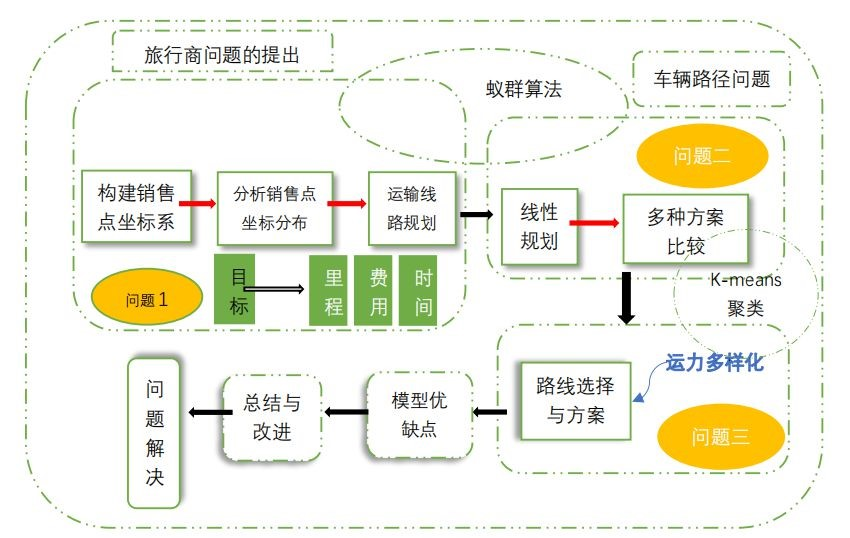
\includegraphics[width=.7\textwidth]{figure/frame.jpg}
        \caption{整体建模框架图}
        \label{fig:frame}
\end{figure}

\section{基本假设}
首先,我们希望为问题做出一些基本假设并作出解释。
\begin{itemize}
    \item {假设一:运输车在任意时刻的前进方向总是平行于两条坐标轴,且忽略运输车转弯时的路径变化。$d_{ij}$为食品销售点i,j之间的几何距离——两个销售点横纵坐标之差的和,
    $$d_{i j}=|x_{i}-x_{j}|+|y_{i}-y_{j}|$$ 
    }
    \item 假设二:每个配送点只会由配送车经过一次。即当配送车到达一个配送点时的卸货量总是一次性满足配送点的需求。这样问题就成了一个多旅行商问题(Multiple traveling salesman problem)。
    \item 假设三:针对需要优化的各项指标,我们考虑的优先级如下:运输总时间>运输总成本>车辆使用数量
\end{itemize}

\section{符号定义与解释}

\begin{center}
    \begin{tabular}{cc}
        \toprule[1.5pt]
        \makebox[0.3\textwidth][c]{符号}	&  \makebox[0.4\textwidth][c]{意义} \\ \midrule
        $n$	    &食品销售点的总个数,本题中为19 \\ 	
        $m$	    &区域划分的数量或运载车总个数\\ 	
        $Path[i]$	    &路径中第i个状态处在的配送站编号,$i=1,2,...,n+1$\\ 
        $distanceMat[i,j]$	    &第i,j个配送站之间的距离,$i,j=1,2,...,n$\\ 
        $x_i,y_i$	    &第$i$个食品销售点的横纵坐标,$i=1,2,...,n$\\ 	
        $D_i$	    &第$i$个食品销售点的需求量,$i=1,2,...,n$\\ 		
        $Z_i$	    &第$i$个食品销售点属于的分区,$i=1,2,...,n$\\ 	
        $L_i$	    &第$i$个运载车的载重量,$i=1,2,...,m$\\ 	
        \bottomrule[1.5pt]
    \end{tabular}
\end{center}


\section{模型的建立与求解}

\subsection{问题1}

    \subsubsection{蚁群算法模型的搭建}

    设$d_{ij}$为食品销售点i,j之间的几何距离(两个销售点横纵坐标之差的和),
        $$d_{i j}=|x_{i}-x_{j}|+|y_{i}-y_{j}|$$ 
    
    每次迭代中,蚂蚁都需要在当前状态选择下一步需要跳转到的状态。在时刻t,蚂蚁k由节点i向节点j的状态转移概率为:
    $$p_{i j}^{k}=\left\{\begin{array}{ll}
        \frac{\tau_{i j}^{\alpha} \eta_{i j}^{\beta}(t)}{\sum_{s \in a \operatorname{alom} d_{k}} \tau_{i s}^{\alpha} \eta_{i s}^{\beta}(t)} & j \in allowed_{k}\\
        0 & \text { else }
        \end{array}\right.$$
    $p_{i j}^{k}$表示在t时刻蚂蚁k由位置i转移到位置j的概率,$allowed_{k}$是未访问过的所有城市集合,$\eta$是启发函数
    $$\eta_{i j}=1/d_{ij}$$

    在每次蚁群迭代完成后,需要更新信息素矩阵。
    $\Delta\tau_{i j}^k$表示 第k只蚂蚁在本次循环中留在ij路径上的信息量,                                 
    $$\Delta \tau_{i j}=\sum_{k=1}^{m} \Delta \tau_{i j}^{k}$$ 
    蚂蚁k,若本次迭代中在第$i,j$两个节点之间跳转过,那么它就对这两个节点之间的信息素有贡献。其对信息素增量的贡献可表达为:
    $$\Delta \tau_{i j}^{k}(t)=\left\{\begin{array}{ll}Q / L_{k} & \text { if the } k _{-} \text {th ant goes through the nodes labeled with i and j on the current iteration } \\ 0 & \text { else }\end{array}\right.$$
    其中$Q$是信息素增益强度。
    $$\tau(i, j) \leftarrow(1-\rho) \tau(i, j)+\rho \Delta \tau(i, j)$$
    其中 $\tau_{i j}$表示t时刻在ij连线上残留的信息量,$\rho$表示信息量的保留度,$\tau_{i j}(0)$是给定常数。

    \begin{figure}[H]
            \centering
            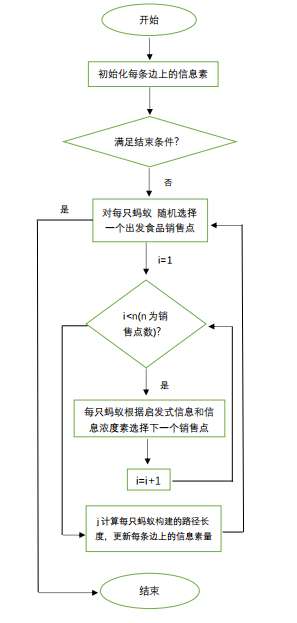
\includegraphics[width=.5\textwidth]{figure/aco.png}
            \caption{蚁群算法流程图}
            \label{fig:aco}
    \end{figure}


    \subsubsection{蚁群算法模型的求解}
    
    模型初始化过程,我们预计算了任意两个配送点之间的距离,组成一个$n\times n$的距离矩阵$distanceMat$,元素$distanceMat[i,j]$表示第$i,j$个配送点之间的距离。\cref{fig:distMat}是矩阵的热图可视化。显然距离矩阵$distanceMat$是一个对称矩阵。

    \begin{figure}[!h]
            \centering
            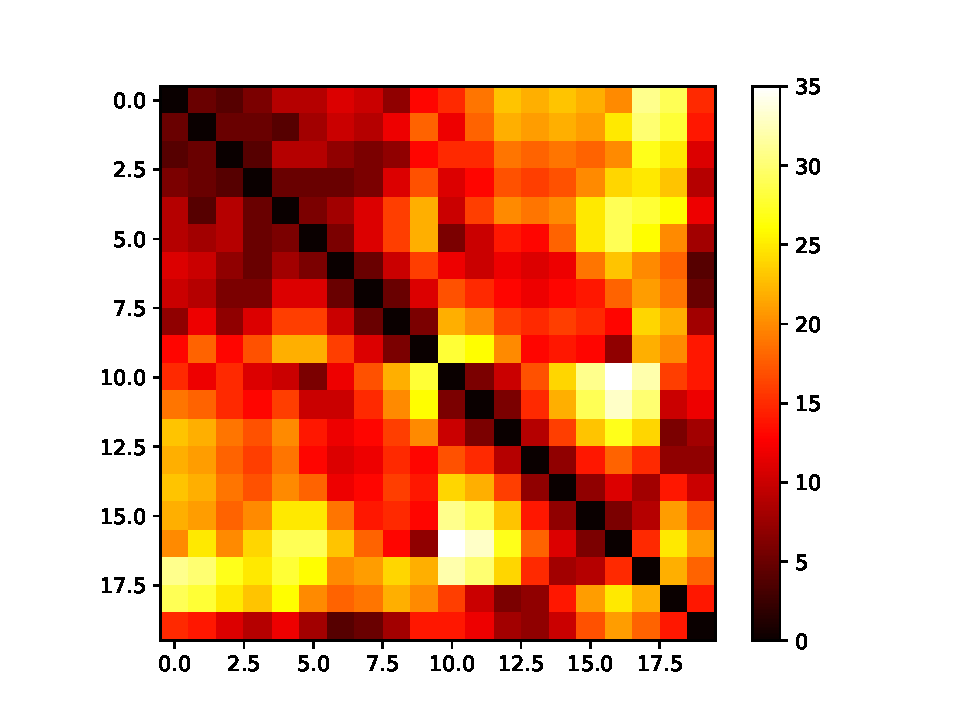
\includegraphics[width=.9\textwidth]{figure/dist_mat_TS.pdf}
            \caption{distanceMat矩阵的热力图可视化}
            \label{fig:distMat}
    \end{figure}

    由于配送点数量较少(仅19),我们蚁群算法选用的蚂蚁个数,最大迭代次数,信息启发式因子,期望启发式因子,信息素挥发速度,信息素强度,如下:

    \begin{table}[!htbp]
        \caption{蚁群算法参数选择}\label{tab:001} 
        \centering
        \begin{tabular}{cccccc}
            \toprule[1.5pt]
            ant\_num & maxIter & alpha & beta & rho & Q \\
            \midrule[1pt]
            40       & 100     & 1     & 5    & 0.1 & 1 \\
            \bottomrule[1.5pt]
        \end{tabular}
    \end{table}
    
    模型的迭代过程,以及给出的解如下:

    \begin{figure}[h]
        \centering
        \begin{minipage}[c]{0.45\textwidth}
            \centering
            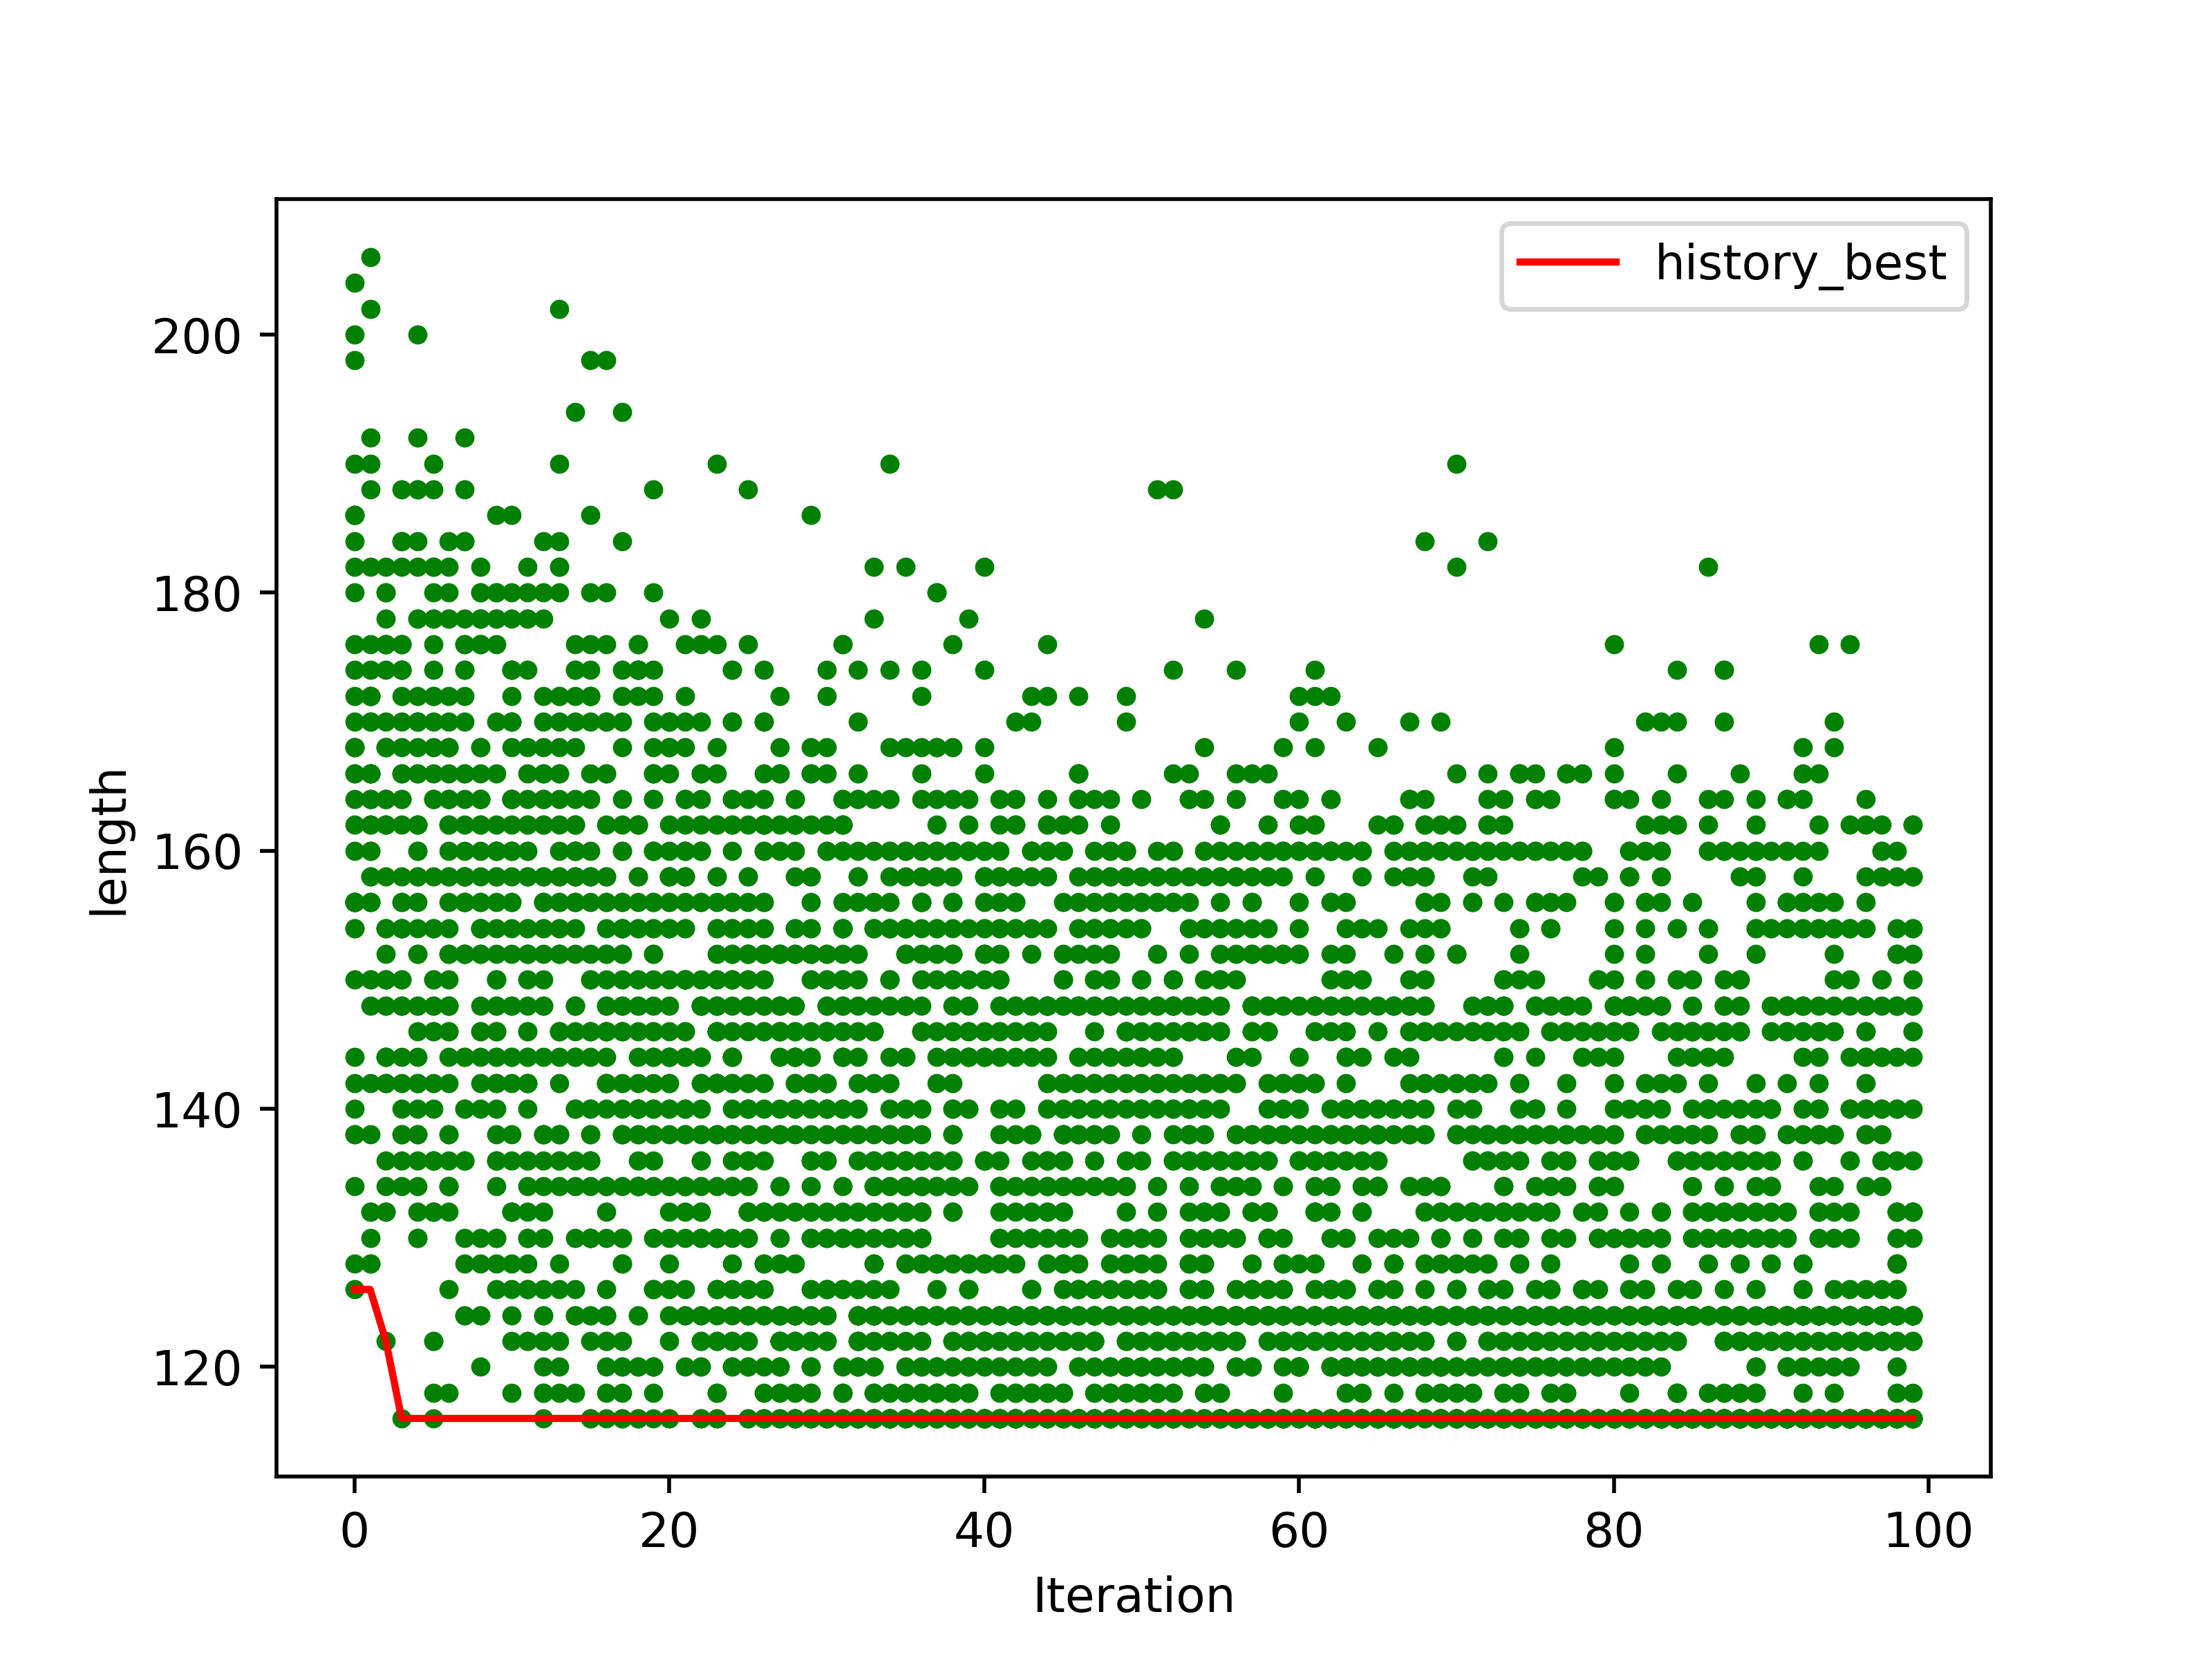
\includegraphics[width=0.95\textwidth]{figure/optimize_process.png}
            \subcaption{蚁群算法优化过程}
            \label{fig:problem1-a}
        \end{minipage}
        \begin{minipage}[c]{0.45\textwidth}
            \centering
            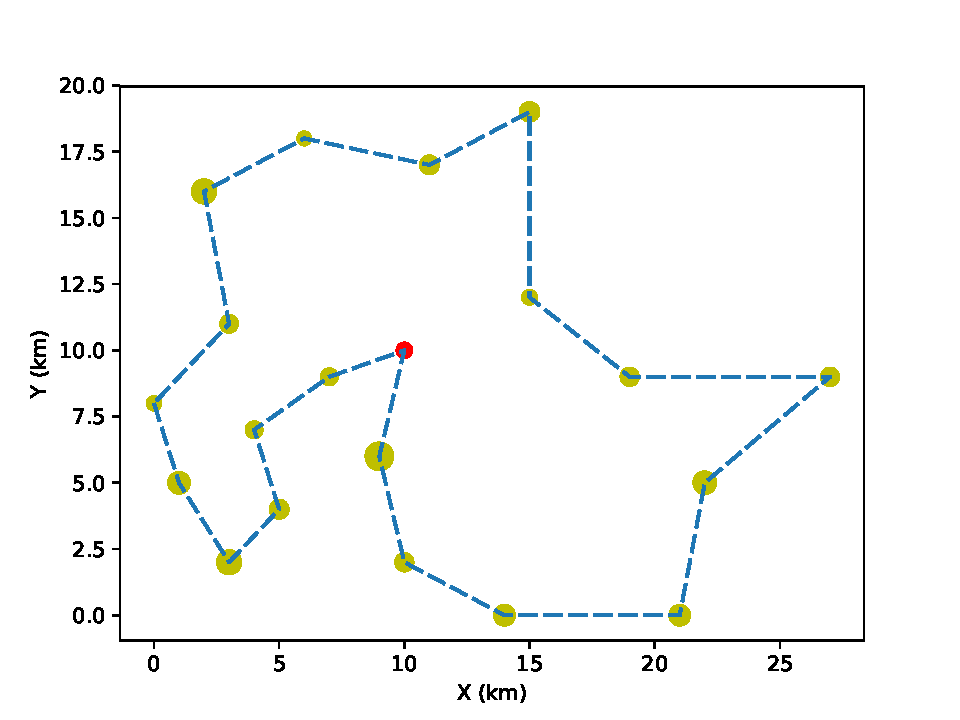
\includegraphics[width=0.95\textwidth]{figure/path_TS.pdf}
            \subcaption{蚁群算法解}
            \label{fig:problem1-b}
        \end{minipage}
        \caption{蚁群算法求解问题1}
        \label{fig:problem1}
    \end{figure}
    注意,\cref{fig:problem1-b}中的虚线并非实际路径,仅展现途径各个配送点的顺序。模型给出的解的路线总长为$116Km$。\cref{fig:problem1-a}中可以看出,经100次迭代总长度已经收敛。

    根据蚁群算法给出的最短路径,我们比较每个环路顺时针运输与逆时针运输时哪一个费用比较少,采用费用少的方案。本题中配送车出发时的总载重量为31.15吨,表达式为:
    $$\sum_{i}^{n} D_i$$
    设求得的路径为$Path$为一个长度为$n+1$列表,若配送站现在处在状态$Path[i]$,那么余下的载重量为:
    $$remainedDemand = \sum_{i,i\in allowed} D_i$$
    其中$allowed$是当前状态下未访问过的配送点。
    计算给定路径费用的表达式为:
    $$\sum_{i=0}^{n} (remainedDemand·loadedCost+noLoadCost)distanceMat[Path[i+1],Path[i]]$$
    计算得\cref{fig:problem1-b}中的总费用为3598元。

\subsection{问题2}
    \subsubsection{概述}
    我们先建立一般化的运输规划模型。
    $n$个食品销售点记为$X_i,i=1,2,...,n$,相应的食品需求量记为$D_{i},i=1,2,...,n$。$m$辆运载车记为$V_i,i=1,2,...,m$, 其载重能力分别为$L_i,i=1,2,...,m$。对于任意应该运输车$V_i$,其执行运输任务$i$所经过的配送点的实际数目记为$N_{i}$,执行一次运输任务所经过的配送点的最大数目记为$\max N_{i}$,则有:
    $$1\leq N_{i} \leq \max N_{i}$$
    记$h_i,i=1,2,...,\max N_{i}$为装载变量,只能取0或1两个布尔值。记$F_i$为执行运输任务$i$出发时的总载重量,则有:
    $$F_i=h_1 D_{Path[1]}+h_2 D_{Path[1]}+...+h_{\max N_{i}}D_{Path[N_{i}]}$$
    其中运输任务$i$的路径$Path$为一个长度为$N_{i}+1$列表.
    显然:
    $$N_i = \sum_{i=1}^{\max N_{i}} h_i$$
    问题二由于涉及多辆配送车。由于运费和当前的载重量有关,所以总运费和总路程并不满足严格的正相关关系。根据假设2,我们将问题2视为多旅行商问题。解决的方法是分3步:
    \begin{itemize}
        \item {将所有配送点划分为$m$类。}
        \item {每个分区使用蚁群算法求解距离最短的路径。}
        \item {比较每个环路顺时针运输与逆时针运输时哪一个费用比较小,采用费用小的方案。}
    \end{itemize}

    \subsubsection{划分方案}
    
    考虑共使用$m$辆运载车,每辆车负责一个区域的配送点,则需要将所有配送点划分为$m$类,即给每个配送点属于的分区一个标记值:
    $$C_1,C_2,...,C_n \in \{c | 0\leq c <m, c\in N\}$$
    属于一个分区的所有配送点需求量之和需要小于运输车的载重,本题中所有运输车都有相同的运载能力,统一记为$L$,每个分区的总需求量需要小于$L$,即需要满足以约束:
    $$\arg\max_{c}\sum_{i,C_i=c }{D_i} \leq L$$
    上式成为区域总需求约束。
    
    直观来说,每个划分的区域要尽量聚集以减少配送车的行驶距离。对于分区的实际操作,我们可以将配送点的横纵坐标视为两个特征,并对配送点进行聚类。聚类方法我们采用经典的k-means算法(k-means clustering algorithm)。k-means是一种基于质心的算法,或基于距离的算法,其目标是最小化簇内点之间的距离。基本流程如下:
    \begin{itemize}
        \item {第一步:选择簇的数目k。}
        \item {第二步:从数据中选择k个随机点作为质心。}
        \item {第三步:将所有点分配给到某个质心距离最近的簇。}
        \item {第四步:重新计算新形成的簇的质心。}
        \item {第五步:重复第三步和第四步,直到新形成的簇的质心不会改变或者达到最大迭代次数。}
    \end{itemize}
    我们可以指定任意的区域数量,但是k-means仅考虑最小化簇内点之间的距离,并不能保证每个区域的总需求量小于运输车的载重量。我们可以用两种方式解决这一问题。
    \begin{itemize}
        \item {方式1:逐渐增多簇的数目k,直至所有的簇均满足区域总需求约束。}
        \item {方式2:选择簇的数目$k_0$后,将所有不满足区域总需求约束的簇再次聚类,细分成$k_m$个簇。直至所有的簇均满足区域总需求约束。其中$k_m$为倍增系数。}
        \end{itemize}

    \subsubsection{模型的求解}
    方式2由于采用聚类数量的倍增,容易使得单个簇的配送点个数过少,我们选择方式1求来解问题2。我们对所有的配送点需求量进行排序后,发现需求量最低的5个配送点的总需求量为5.95,所以每个区域的配送点数量都小于等于5,那么区域划分的数量$m$至少为4。我们尝试了k-means 簇的个数为$m\in\{4,5,6,7,8,9\}$进行实验。模型给出的聚类结果,以及相应的路径如\cref{fig:path_mutiTS}。

    \begin{figure}[H]
        \centering
        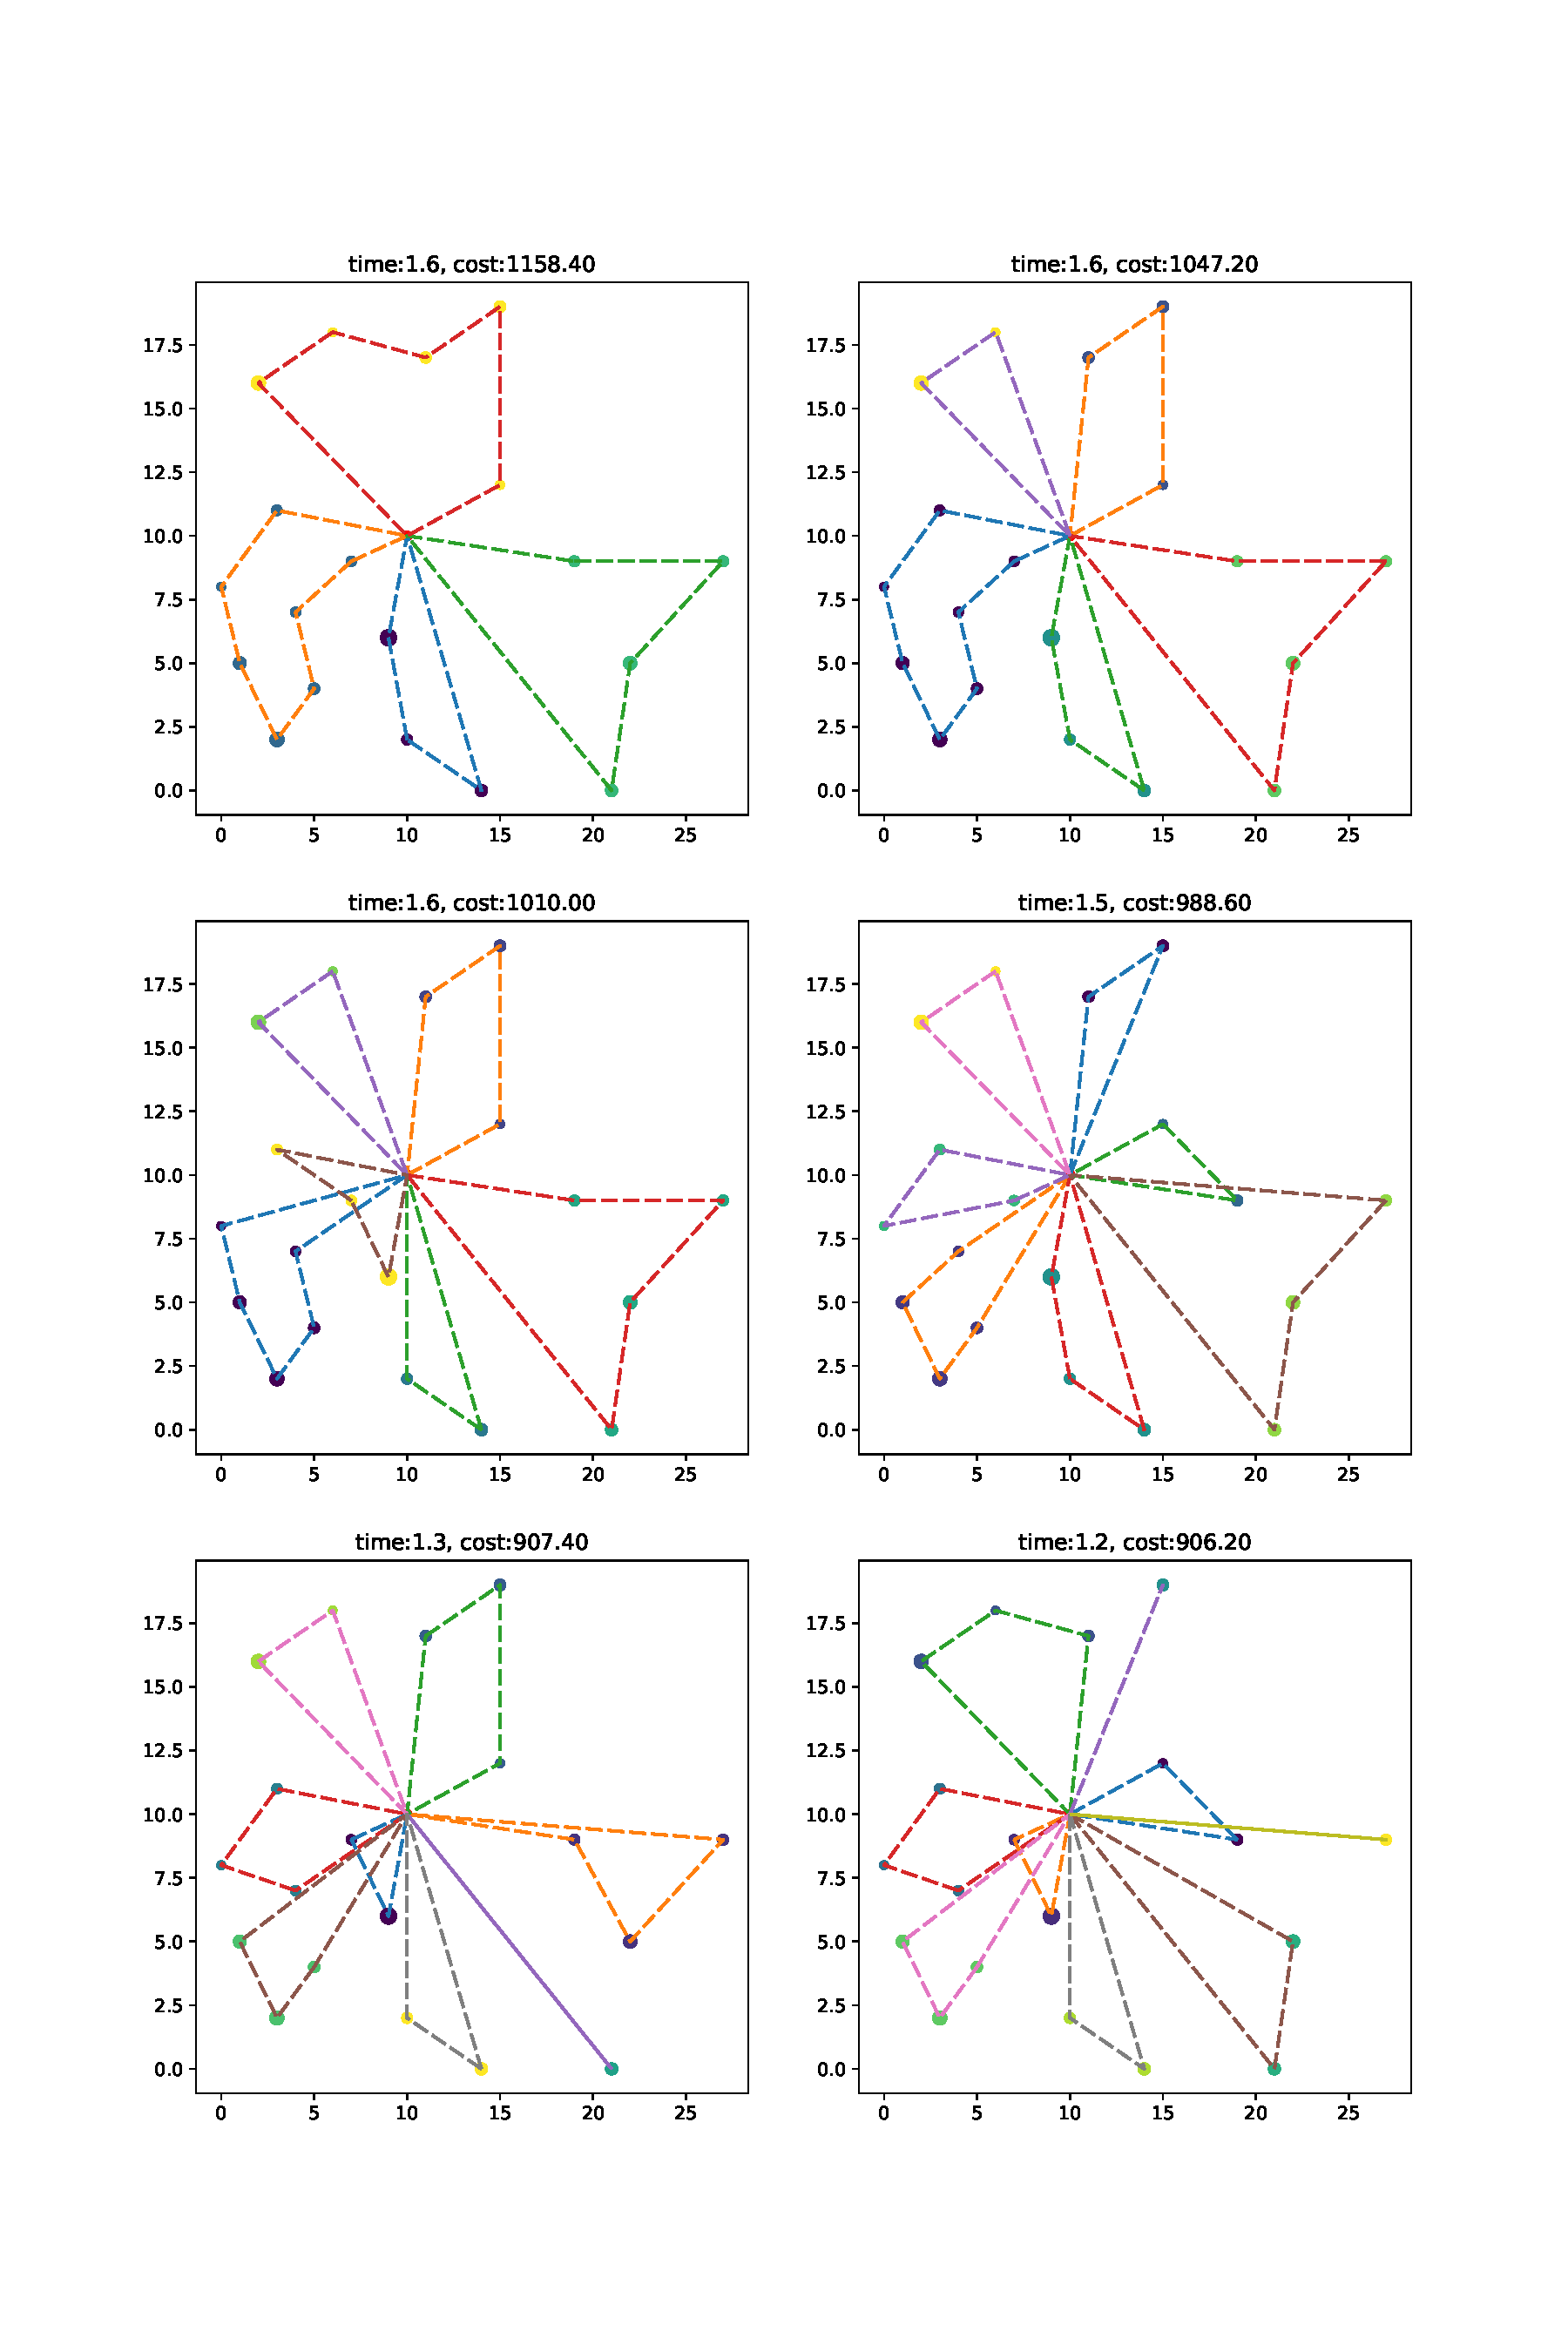
\includegraphics[width=.95\textwidth]{figure//path_mutiTS_6pic.pdf}
        \caption{聚类结果和路径}
        \label{fig:path_mutiTS}
    \end{figure}

    可以直观的看出各区域内部的配送点相对聚集,接下来我们验证这些区域划分是否满足区域总需求约束,\cref{fig:distance_cost_line}可视化各种分区方式的总路程和总费用。

    \begin{figure}[H]
        \centering
        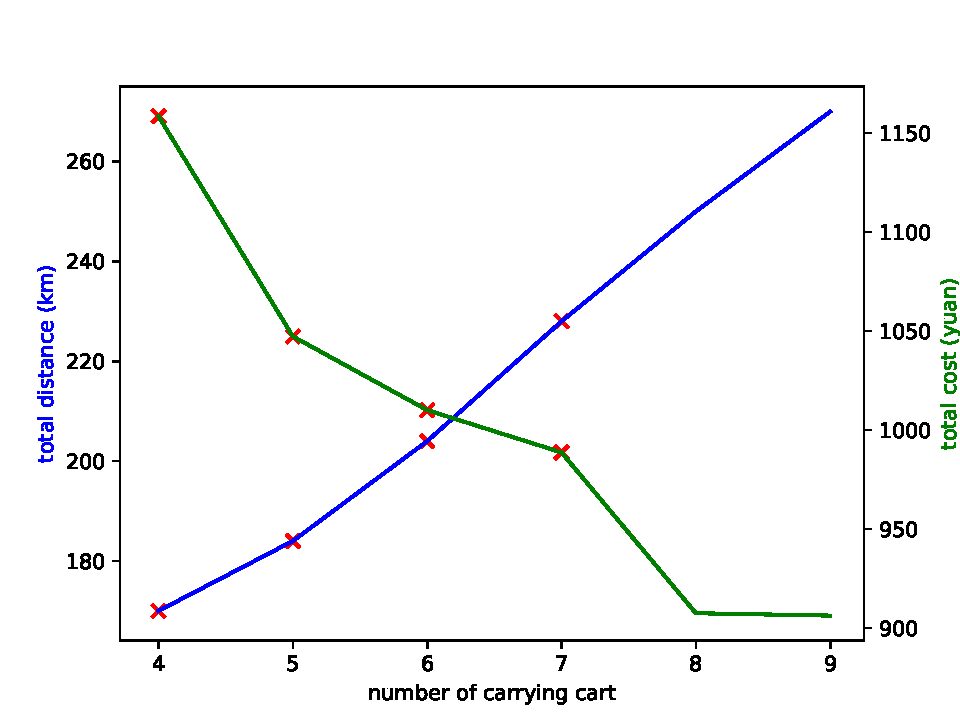
\includegraphics[width=.7\textwidth]{figure//distance_cost_line.pdf}
        \caption{各分区总路程和总费用}
        \label{fig:distance_cost_line}
    \end{figure}

    \cref{fig:distance_cost_line}中数据点的红色"x"表示该划分方式不满足区域总需求约束,即划分4到7个区域时,总需求量最大区域的需求量均超过了运载车最大载重量6吨,只有分区为8,9两个可行方案。\cref{fig:distance_cost_line}中折线的趋势表明,划分的区域数量越多,运载车运行的总路程增加,总成本降低。

    \begin{figure}[H]
        \centering
        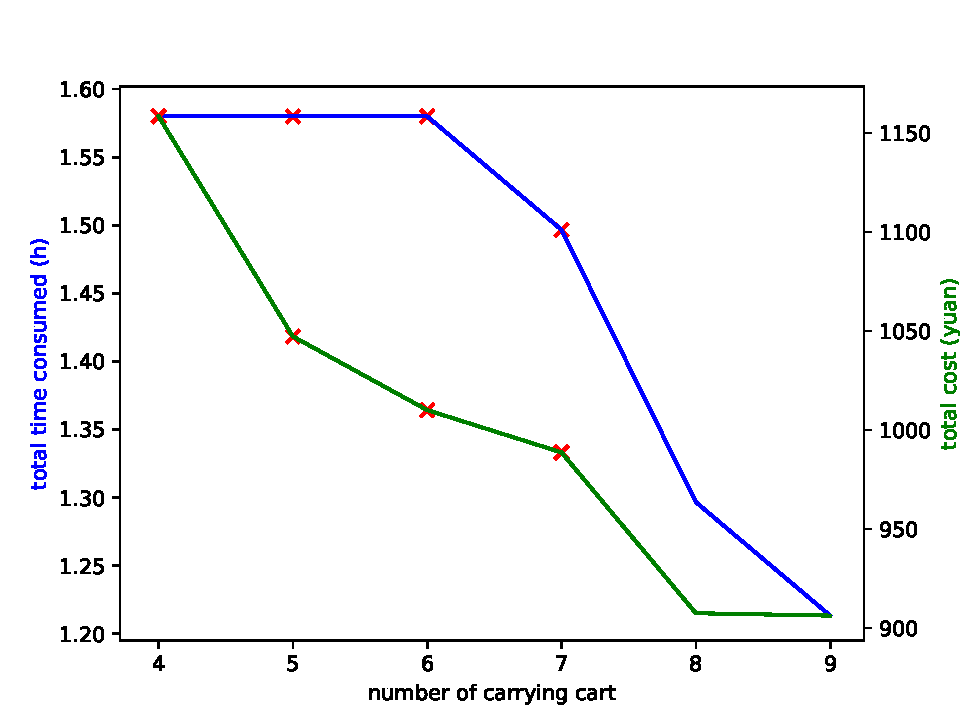
\includegraphics[width=.7\textwidth]{figure//time_cost_line.pdf}
        \caption{配送总时间和总费用}
        \label{fig:time_cost_line}
    \end{figure}

    \cref{fig:time_cost_line}中折线的趋势表明,划分的区域数量越多,所以运载车花费的最大时间(即配送完成的总时间)减少。
    对比可行的分区为8,9两个可行的方案。

    \begin{table}[!h]
        \caption{可行方案对比}\label{tab:001} \centering
        \begin{tabular}{cccc}
            \toprule[1.5pt]
            $m$(in) & total time consumed(h) & total cost (yuan) & total distance(km) \\
            \midrule[1pt]
            8 & 1.5 & 907.4 & 250.0\\
            9 & 1.3 & 906.2 & 270.0\\
            \bottomrule[1.5pt]
        \end{tabular}
    \end{table}

    由\cref{tab:001},9量运载车使用的总时间比8量减少了13.3\%,而总费基本相同,所以综合考虑时和费用因素,使用9量运载车更优。

\subsection{问题3}
    \subsubsection{概述}
    问题三中提供了载荷能力分别为4吨和6吨的两种运输车,两类车在空载时的费用不一样,分别为0.2元/公里和0.4元/公里。在问题二中我们讨论过总费用与总路程的关系,显然,在载荷能力满足运输要求的情况下,选择4吨级运输车在费用方面更有优势。我们对该问题的解决方法仍分三部分:

    \begin{itemize}
        \item 将所有配送点划分为 m 类
        \item 每个分区使用蚁群算法求解距离最短的路径
        \item 比较每个环路顺时针运输与逆时针运输时哪一个费用比较小,采用费用小的方案。
    \end{itemize}

    \subsubsection{划分方案}
    面对新的运力情况,我们仍可以指定任意的区域数量,在问题二有关K-means方法划分的基础上,我们希望进一步改进。
    记本题中运载能力分别为4吨和6吨的两种运输车的载荷分别为$L_1$和$L_2$,每个分区的总需求需要小于对应的运输载荷。即需要满足约束:
    $$\max_{c}\sum_{i,C_i=c }{D_i} \leq \max(L_1, L_2)$$

    问题二中我们已经讨论过簇的划分方案,其核心思想是保证在任意簇中运输需求满足相应约束条件。本题中不同的是,我们有两种运力载荷的配送车。本题我们采用倍增的k-means簇数量来进行分区。流程如下:
    \begin{itemize}
        \item k-means倍增分区策略:选择簇的数目$k_0$后,将所有不满足区域总需求约束的簇再次聚类,细分成$k_m$个簇。直至所有的簇均满足区域总需求约束。
        \item 对每个区域分配运载车:若该区域的总食品需求在[0,4]吨内,我们选择派出运载能力为$L_1$的运输车执行任务;若该区域的总食品需求在(4,6]吨内,我们选择派出运载能力为$L_2$的运输车执行任务。
        \item 每个分区使用蚁群算法求解距离最短的路径。
        \end{itemize}
  

    \subsubsection{模型的求解}
    \cref{fig:path_mutiTSSheet2}展示了最终递归分区的聚类结果和蚁群算法输出的路径。经验证,次方案满足区域总需求约束。最终的总运费为896.6元,总运输时间为1.297小时,所有运输车行驶的总距离为216千米。
    \begin{figure}[!h]
        \centering
        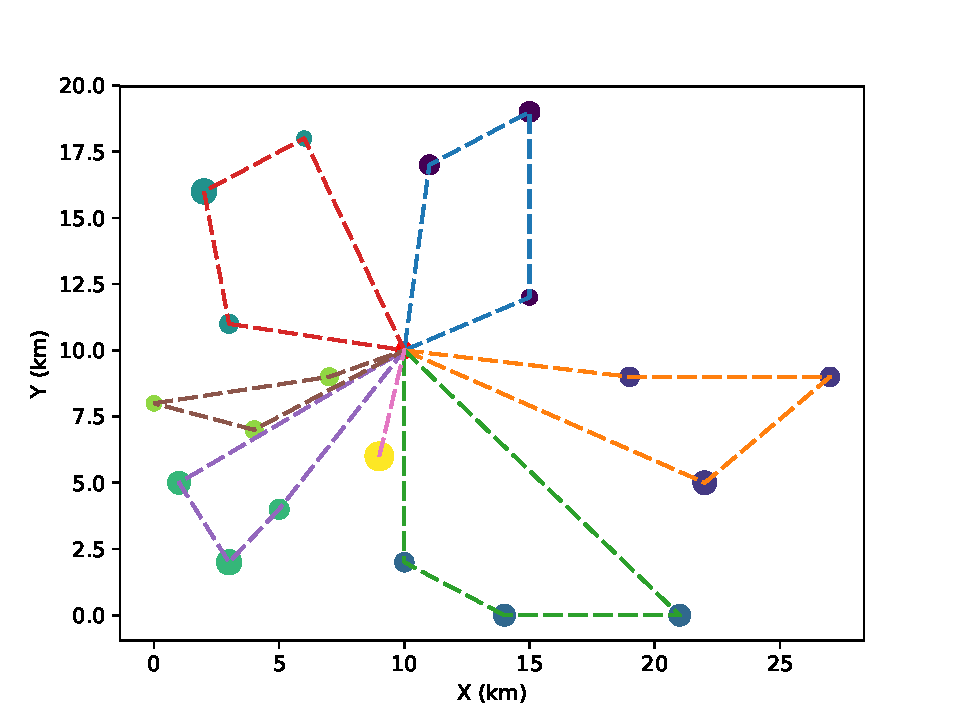
\includegraphics[width=.7\textwidth]{figure//path_mutiTSSheet2.pdf}
        \caption{倍增的k-means分区路径}
        \label{fig:path_mutiTSSheet2}
    \end{figure}

    本分区方案中,个簇的需求量和分配的配送车载重量见\cref{tab:002}。可以得出次方案需要4辆载重量为6吨的,和3辆载重量为4吨的运载车。
    \begin{table}[!htbp]
        \caption{需求量和分配的配送车载重量}\label{tab:002} \centering
        \begin{tabular}{ccccccc}
            \toprule[1.5pt]
            1 & 2 & 3 & 4 & 5 & 6 & 7\\
            \midrule[1pt]
            4.0 & 5.0 & 5.0 & 4.6 & 6.0 & 3.25 & 3.3 \\
            4 & 6 & 6 & 6 & 6 & 4 & 4 \\
            \bottomrule[1.5pt]
        \end{tabular}
    \end{table}

\newpage

\section{模型优缺点}
    \subsection{模型的优点}
    \begin{itemize}
        \item 模型分区和求解路径的过程流程清晰,对配送点的各种分布情况鲁棒性强,配送点分区过程的人为设定少。
        \item 蚁群算法作为一种启发式算法,可以通过正反馈式的信息传递和积累,快速寻优,且由于算法的早熟性收敛可以通过其分布式计算特征加以避免,同时具有良好的全局优化特征。
        \item 具有贪婪启发式搜索特征的蚁群系统又能在搜索过程的早期找到可以接受的问题解答。
    \end{itemize}

    \subsection{模型的不足}
    \begin{itemize}
        \item k-means算法本身仅考虑配送点位置,对需求量因素并未考虑,所以每个分区的总需求量不可控。
        \item 蚁群算法的核心是寻找一个较好的局部最优解,因为在面临大量数据点时可能找不到全局最优解,且开始时算法收敛速度较快,一旦迭代超过一定次数,容易出现停滞。
        \item 蚁群算法的稳定性较差,即使参数不变,每次执行程序也容易出现不同的解。
    \end{itemize}

\section{总结与改进}
\subsection{建模过程总结}
为了对本车辆路径优化问题进行求解,我们构建了一个基于蚁群算法的组合优化模型,在需求点数较少且约束情况比较宽松的情况下,我们的模型能够较快的找出一个最优解,在进行多种线路条件下的汽车的调运时,我们使用K-means聚类方法能够较好的为离散的需求点进行归类,有效的减少了计算量。同时,我们对大量可行解做出了充分比较,得到了复杂约束条件下的一个可接受规划。
\subsection{未来改进方向}

\begin{itemize}
    \item 在实验中蚁群算法的相关超参数并未进行调优,而是始终采用了一组确定值,可以进一步考虑模型超参数的调优策略。
    \item 由于k-means聚类的结果跟随初始化的质心位置有关,且蚁群算法给出解也具有不稳定性,所以下一步可以多次执行以寻找最佳解。
    \item 可以在k-means迭代过程中手动设置一些规则,把配送点的需求量纳入考虑,使得分区的总需求量尽量可控。
    \item 若k-means的分区结果只有少量不满足区域总需求约束。
\end{itemize}

\section{参考文献}

[1]王芹. 带时间窗的冷链食品物流配送选址及运输路径优化问题研究[D].长安大学,2015.

[2]李雪,王雷.改进蚁群算法在解决TSP问题中的应用[J].宜春学院学报,2020,42(03):63-67.

[3]叶家琪,符强,贺亦甲,叶浩.基于聚类集成的蚁群算法求解大规模TSP问题[J].计算机与现代化,2020(02):31-35.

[4]冯志雨,游晓明,刘升.基于自适应更新策略的蚁群算法在TSP上的应用[J].测控技术,2019,38(10):66-70+75.

[5]罗梓瑄,刘学文.基于蚁群算法的物流配送路径优化研究[J].重庆工商大学学报(自然科学版),2020,37(04):89-94.

[6]邓学平,孙芹,田帅辉.基于不同车型的城市快递配送车辆路径优化研究[J].价值工程,2020,39(12):275-280.


\begin{appendices}
		
\section{PYTHON 源程序}
\subsection{蚁群算法主体}
\begin{lstlisting}[language=Python]%设置不同语言即可。
class ACO(object):
    def __init__(self, ant_num=40, maxIter=100, alpha=1, beta=5, rho=0.1, Q=1, df=None):
        self.ants_num = ant_num   # 蚂蚁个数
        self.maxIter = maxIter    # 蚁群最大迭代次数
        self.alpha = alpha        # 信息启发式因子
        self.beta = beta          # 期望启发式因子
        self.rho = rho            # 信息素挥发速度
        self.Q = Q                # 信息素强度
        #  提取所有城市的坐标信息
        if df is None:
            self.df = read_data.read_data()
        else:
            self.df = df
        self.deal_df(self.df)
        ###########################
        self.path_seed = np.zeros(self.ants_num).astype(int)      # 记录一次迭代过程中每个蚂蚁的初始城市下标
        self.ants_info = np.zeros((self.maxIter, self.ants_num))  # 记录每次迭代后所有蚂蚁的路径长度信息
        # 记录每次迭代后整个蚁群的“历史”最短路径长度,和该路径的总运费
        self.best_length = np.zeros(self.maxIter)
        self.best_cost = 0
        ###########################
        # self.solve()              # 完成算法的迭代更新
        # self.display()            # 数据可视化展示

    def deal_df(self, df):
        self.cities_num = len(df)                                                   # 1. 获取城市个数
        #  2. 构建城市列表
        self.cities = np.array(df[["X", "Y", "requirement"]])
        self.city_dist_mat = np.zeros((self.cities_num, self.cities_num))                  # 3. 构建城市距离矩阵
        for i in range(self.cities_num):
            self.city_dist_mat[i] = np.abs(self.cities[i, 0] - self.cities[:, 0]) \
                                    + np.abs(self.cities[i, 1] - self.cities[:, 1])
        plot.plot_mat(self.city_dist_mat, name="dist_mat_TS")
        self.phero_mat = np.ones((self.cities_num, self.cities_num))                       # 4. 初始化信息素矩阵
        # self.phero_upper_bound = self.phero_mat.max() * 1.2                              #b信息素浓度上限
        self.eta_mat = 1/(self.city_dist_mat + np.diag([np.inf]*self.cities_num))          # 5. 初始化启发函数矩阵

    def solve(self, save_img_name=None, verbose=False):
        for iterNum in tqdm(range(self.maxIter)) if show_progress else range(self.maxIter):
            self.random_seed()                                                 # 使整个蚁群产生随机的起始点
            delta_phero_mat = np.zeros((self.cities_num, self.cities_num))     # 初始化每次迭代后信息素矩阵的增量
            for i in range(self.ants_num):
                city_index1 = self.path_seed[i]                                # 每只蚂蚁访问的第一个城市下标
                ant_path = Path(self.cities[city_index1], self.cities_num)     # 记录每只蚂蚁访问过的城市
                tabu = [city_index1]                                           # 记录每只蚂蚁访问过的城市下标,禁忌城市下标列表
                non_tabu = list(set(range(self.cities_num)) - set(tabu))
                for j in range(self.cities_num-1):                             # 对余下的城市进行访问
                    up_proba = np.zeros(self.cities_num-len(tabu))             # 初始化状态迁移概率的分子
                    up_proba = np.power(self.phero_mat[city_index1][non_tabu], self.alpha) * \
                        np.power(self.eta_mat[city_index1][non_tabu], self.beta)
                    proba = up_proba/sum(up_proba)                             # 每条可能子路径上的状态迁移概率
                    proba_cumsum = np.cumsum(proba)
                    # 提取出下一个城市的下标
                    choicesArr = np.where(proba_cumsum > np.random.rand())[0]
                    if choicesArr.size == 0:
                        choice = -1
                    else:
                        choice = choicesArr[0]
                    city_index2 = non_tabu[choice]

                    ant_path.add_path(self.cities[city_index2])
                    tabu.append(city_index2)
                    non_tabu = list(set(range(self.cities_num)) - set(tabu))
                    city_index1 = city_index2
                self.ants_info[iterNum][i] = Ant(ant_path.path).calc_length()
                if iterNum == 0 and i == 0:                                    # 完成对最佳路径城市的记录
                    self.best_cities = ant_path.path
                else:
                    if self.ants_info[iterNum][i] < Ant(self.best_cities).calc_length():
                        self.best_cities = ant_path.path
                tabu.append(tabu[0])                                           # 每次迭代完成后,使禁忌城市下标列表形成完整闭环
                for l in range(self.cities_num):
                    delta_phero_mat[tabu[l]][tabu[l+1]] += self.Q/self.ants_info[iterNum][i]

            self.best_length[iterNum] = Ant(self.best_cities).calc_length()
            self.update_phero_mat(delta_phero_mat)                             # 更新信息素矩阵
        best_ant = Ant(self.best_cities)
        self.best_cost = best_ant.calc_cost()
        self.total_time = best_ant.calc_time()
        if save_img_name is not None:
            plot.display_TS(self.df, save_img_name, self.ants_info, self.best_length, self.best_cities)
        if verbose:
            print("\nbest result: {} {}.\n".format(self.best_length[-1], self.best_cost))
        return self.best_length[-1], self.best_cost, self.total_time

    def update_phero_mat(self, delta):
        self.phero_mat = (1 - self.rho) * self.phero_mat + delta

    def random_seed(self):                                                     # 产生随机的起始点下表,尽量保证所有蚂蚁的起始点不同
        if self.ants_num <= self.cities_num:                                   # 蚂蚁数 <= 城市数
            self.path_seed[:] = np.random.permutation(range(self.cities_num))[:self.ants_num]
        else:                                                                  # 蚂蚁数 > 城市数
            self.path_seed[:self.cities_num] = np.random.permutation(range(self.cities_num))
            temp_index = self.cities_num
            while temp_index + self.cities_num <= self.ants_num:
                self.path_seed[temp_index:temp_index + self.cities_num] = np.random.permutation(range(self.cities_num))
                temp_index += self.cities_num
            temp_left = self.ants_num % self.cities_num
            if temp_left != 0:
                self.path_seed[temp_index:] = np.random.permutation(range(self.cities_num))[:temp_left]

\end{lstlisting}
\subsection{路径,和蚂蚁类}
\begin{lstlisting}[language=Python]

class Ant(object):# 建立“蚂蚁”类
    def __init__(self, path):
        self.path = path                       # 蚂蚁当前迭代整体路径
        self.unload_time = 1/12                #下货时间
        self.speed = 50                        #平均速度 km/h

    def permutation_path(self):
        # path=[A, B, C, D, A]注意路径闭环,将路径重新排列成配送站为出发点(A)
        permuted = np.zeros_like(self.path)
        warehouseID = np.where(self.path[:, 2] == 0)[0][0]
        pathSize = self.path.shape[0]
        permuted[:(pathSize-warehouseID)] = self.path[warehouseID:]
        permuted[(pathSize-warehouseID):]= self.path[1:warehouseID+1]
        self.path = permuted

    def calc_length(self):
        # 计算路径的总长度
        length = 0
        for i in range(len(self.path)-1):
            delta = np.abs(self.path[i, 0] - self.path[i+1, 0]) + np.abs(self.path[i, 1] - self.path[i+1, 1])
            length += delta
        return length

    def calc_time(self):
        # 计算路径的配送时间
        return self.calc_length()/self.speed + self.path.shape[0] * self.unload_time

    def calc_cost(self, has_small_cart=True):
        # 计算路径的总费用
        if self.path[0, 2] != 0:
            self.permutation_path()
        self.loaded_cost = 2
        self.total_demand = np.sum(self.path[:, 2])
        if self.total_demand <= 4 and has_small_cart:
            self.no_load_cost = 0.2
        elif self.total_demand <= 6:
            self.no_load_cost = 0.4
        else:
            self.no_load_cost = 0.6

        cost0, cost1 = 0, 0
        load = self.total_demand
        for i in range(len(self.path)-1):
            delta = np.abs(self.path[i, 0] - self.path[i+1, 0]) + np.abs(self.path[i, 1] - self.path[i+1, 1])
            if load > 1e-5:
                delta_cost = load * self.loaded_cost * delta
            else:
                delta_cost = self.no_load_cost * delta
            load -= self.path[i+1, 2]
            cost0 += delta_cost
        load = self.total_demand
        self.path = self.path[::-1, :]# 倒序排列
        for i in range(len(self.path)-1):
            delta = np.abs(self.path[i, 0] - self.path[i+1, 0]) + np.abs(self.path[i, 1] - self.path[i+1, 1])
            if load > 1e-5:
                delta_cost = load*self.loaded_cost * delta
            else:
                delta_cost = self.no_load_cost *delta
            load -= self.path[i+1, 2]
            cost1 += delta_cost
        return min(cost0, cost1)

class Path(object):# 建立“路径”类
    def __init__(self, A, cities_num):                     # A为起始城市
        self.path = np.zeros((cities_num+1, 3))
        self.path[0] = A
        self.path[-1] = A
        self.step = 1

    def add_path(self, B):                     # 追加路径信息,方便计算整体路径长度
        self.path[self.step] = B
        self.step += 1
\end{lstlisting}
\end{appendices}

\end{document} 